\addtocontents{toc}{\protect}
\section{\texorpdfstring{\MakeUppercase{the mcfacts code: monte carlo method for black hole mergers in agn disks}}{the mcfacts code: monte carlo method for black hole mergers in agn disks}}
\label{sec:apdx-mcfacts}

\counterwithin{figure}{section}
\counterwithin{table}{section}

The contents of this appendix was published in \citet{McKernan+25-mcfactsI}. Please use that reference when citing this section.

Fig.~\ref{fig:overview} gives a basic overview of the flow of BH through categories in \code{McFACTS}, starting from an initial eccentric BH population of singleton BH in the AGN disk (top left).
Solid arrows indicate a flow from one category to another and dotted arrows indicate influence from one category on another.
For example, there is a flow from the initial eccentric BH population into the circularized BH population via gas damping (blue solid arrow), but the eccentric BH population also dynamically interacts with the circularized population (dotted red arrow) and can excite it to reverse the flow (solid red arrow).
Binary BH are formed from among the circularized population (connecting solid red arrow).
BBH, once formed can dynamically interact with both the eccentric and circularized single BH and the spheroid population (the three dotted red arrows onto Binary BH in Fig.~\ref{fig:overview}).
BBH can flow to softer BBH and ionize, via dynamics (solid red arrows) returning their components back to the eccentric disk BH population, but BBH can also harden via gas and dynamics (blue and red arrows) and ultimately merge, whereupon they either flow back into the eccentric BH population or into the spheroid (from where they can be re-captured generally circularized).
A small sub-population of the initial eccentric population and the spheroid population can flow into the inner disk, where some BH can decay via GW emission and become EMRIs (blue box).
\begin{figure*}
	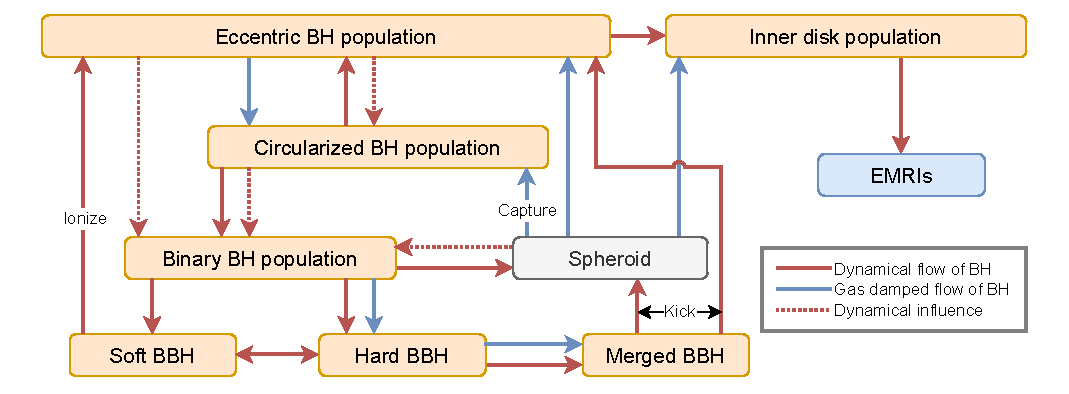
\includegraphics[width=1\textwidth]{appdx_figs/McFacts_flowchart.pdf}
	\caption[Flow diagram of BH categorization in \code{McFACTS}]{Flow diagram indicating how BH are categorized in \texttt{McFACTS} and how BH are exchanged between these categories. Solid arrows indicate a flow of objects from one category to another and dotted arrows indicate an influence of one category on another. Red denotes dynamics, blue denotes gas. Objects in orange (grey) boxes are in the disk (spheroid). EMRIs are in the blue box. For example, there is a flow from the initially eccentric BH population to the circularized BH population due to gas damping (blue arrow), but the eccentric BH population also has a dynamical influence on the circularized BH population (red dotted line) leading to a reverse flow (red solid line). 
    }
    \label{fig:overview}
\end{figure*}

Objects in their disks have their physical parameters manipulated in a consistent algorithmic manner via the \verb|AGNObject| class.
This class will be extended from just BH to stars, neutron stars, and white dwarfs in future updates to the code.
Each \verb|AGNObject| is given a unique ID number, stored in an instance of the \verb|AGNFilingCabinet| class, along with other parameters such as the object's mass and location in the AGN disk.
This allows the code to iterate over the entire population of disk objects when calculating e.g. interactions and binary formation, rather than separating and evaluating objects by type for each iteration.

\subsection{Initial conditions and other inputs}
There are three basic inputs for any simulated galactic nucleus: the SMBH, the NSC, and the AGN disk.
The initial conditions for each of these is set via an input file, for which a default file is provided, or constructed by the user (see Table~\ref{tab:default_model} for \code{p1_default_model.ini}).
Primary input parameters are the SMBH mass ($M_{\rm SMBH}$), the NSC mass ($M_{\rm NSC}$) and the AGN disk model type---users may choose from either a \cite{SirkoGoodman03} or \cite{ThompsonQuataertMurray05} type disk, as implemented in the \code{pAGN} package \citep{Gangardt+24-pAGN} (and for which the user must also specify the disk $\alpha$ parameter, mass accretion rate, $\dot{m}$, and radiative efficiency $\eta$), or may supply their own disk model if they can provide tabulated surface density ($\Sigma$), aspect ratio ($h/r$), and opacity ($\tau$) profiles as a function of disk radius (subject to the requirement that a user-supplied model must be interpolatable over the range of disk radii under consideration, see also below).
A simplified implementation of both the \cite{SirkoGoodman03} and \cite{ThompsonQuataertMurray05} disk models which assumes constant opacity is also provided in \code{McFACTS} along with the pAGN implementation.

We do not currently consider the spin of the SMBH, so there are no input parameters related to it.
However the NSC and the AGN disk have a number of important additional parameters that the user can specify (or use the defaults provided).
Given $M_{\rm NSC}$ and a disk model, we determine (purely based on geometry) the number of stellar mass black holes with orbits fully embedded in the AGN disk at the time the AGN disk initially arrives in the nucleus (here we make the simplifying assumption that the disk does not evolve through the simulation, appearing instantaneously at time zero, subsequently vanishing instantaneously at time $\tau_{\rm AGN}$, the lifetime of the AGN disk, also specified in the input file).
The remainder of the NSC parameters are for distribution functions from which we select the actual objects included in a given simulation for each galaxy.
The user can specify a random number seed (\code{SEED}) in the \code{Makefile} or take the default (in either case the value is recorded for reproducibility).
If the user is simulating multiple galaxies with the same input parameters (the usual mode of operation, in order to build up statistics), each new galaxy will (by default) iterate the original random seed by one, ensuring an entire suite of simulations can be easily reproduced from a starting \code{SEED} and \code{.ini} file.

The \code{SEED} is used to generate initially embedded stellar black hole (BH) masses, orbital semi-major axes ($a$), eccentricities ($e$), inclinations ($i$), arguments of periapse ($\omega$), spin magnitude ($\chi$), and spin angle ($\theta$) from initial distributions set by the \code{.ini} file.
BH masses are drawn from an initial mass function (IMF), assumed to be a Pareto function with a mode mass and powerlaw slope, each of which the user can specify in the \code{.ini} file.
An additional mass feature can be added to the IMF by piling up masses drawn from the powerlaw IMF beyond some maximum mass in a user specified Gaussian distribution.
In this way we can emulate a possible pair instability supernova (PISN) bump in the BH IMF, as physically expected from models of stellar evolution \citep[e.g.][]{RenzoSmith24}, as well as a mass pile-up in the LVK observations \citep{Abbott+23-massbump}.
BH number density is set by the NSC model and default is a broken power-law distribution consistent with NSC models \citep{Generozov+18,NeumayerSethBoker20}.
The number of BH geometrically coincident with the disk between disk inner and outer radii is then calculated and BH orbital semi-major axes are chosen from a (default) broken power law distribution consistent with the NSC radial density distribution, although the user can also draw from a uniform distribution.
Orbital eccentricities are drawn uniformly between zero and a (user specified) maximum initial eccentricity by default but the user can also specify a thermal initial distribution (likely the limiting case where a population has fully relaxed between AGN episodes).
Orbital inclinations of embedded BH are selected uniformly between $\pm h/r$, the disk aspect ratio, where $h$ is the disk height from the midplane at radius $r$. 

Next we assign an orbital angular momentum flag of $\pm 1$ to specify either prograde or retrograde orbits with respect to the disk gas, allowing us to apply appropriate physics to the different objects (and implicitly setting the inclinations to be either $i=0\pm h/r$ (prograde) or $i=\pi \pm h/r$ (retrograde)) where orbiters with $i=0^{\circ}$ lie prograde in the disk midplane.
The argument of periapse for each object is currently chosen to be either $0$ or $\pi/2$ (see \S\ref{sec:singlebh} below).
We recognize this is a limitation of the code as the timescales for capture depend strongly on the argument of periapse and differ by orders of magnitude between these two values.
This decision will overestimate the capture efficiency at early times, and underestimate the capture efficiency at late times, but over the course of a typical run, these behaviors should roughly average out in the population statistics.
\footnote{In reality a random distribution across a wider range of values would be more appropriate; however, the form of the evolution of an orbiter is also quite disparate between these two values.
Interpolating between them, or, for even greater precision, passing the orbital parameters to an N-body code, would add substantial computational expense, so we currently leave the two extremal behaviors as the only options.
We plan to add \textit{slightly} finer divisions in a future release}.
BH spin magnitude (dimensionless spin parameter) is chosen from a Gaussian distribution defined by a user specified mean and standard deviation.
BH spin angles ($\theta$, w.r.t. the AGN disk orbital angular momentum) are chosen uniformly between $[0,\pi/2]\,([\pi/2,\pi])$(radians) for BH with initial positive (negative) spin parameters, where $\theta=0(\pi)$ is fully aligned(anti-aligned) with the AGN disk gas.
If the disk model is expected to contain a migration trap, the user must specify the radius.
A disk outer radius must also be specified, with the default disk inner radius assumed to be the innermost stable circular orbit (ISCO) for a non-spinning (Schwarzschild) SMBH. 

Finally, the user must specify the duration of a timestep in years and the number of timesteps per galaxy, the product of which specifies the total disk lifetime ($\tau_{\rm AGN}$, plausibly $\sim 0.1-10{\rm Myr}$).
A default timestep duration of $10^{4}$ yr provides a reasonable compromise between computational speed and the resolution of the physical processes being modeled.
Users who wish to see finer detail on particular physical processes or individual events may choose smaller timesteps. 

\subsubsection{Physical processes modelled}

\subsubsubsection{Single BH in the disk}
\label{sec:singlebh}
For every galaxy, we compute the number of black holes which should be coincident with the AGN disk, based on the user specified parameters for the disk and NSC, based on geometry.
We then draw the requisite number of black holes from the distributions specified by the user and find, for their orbit around the SMBH, a semi-major axis, eccentricity, inclination and argument of periapse; we also find the mass, spin, and spin angle for each object.
The initial binary fraction is zero, so all binaries in the simulation must be formed dynamically.
We will allow for a user-specified initial binary fraction in future code updates. 

We then distinguish between prograde and retrograde orbiters, as they are subject to different processes.
We also separate out the innermost disk orbiters (set by default to objects with semi-major axes $<50\,r_{g}$, adjustable by the user).
We evolve orbits of inner disk objects\footnote{The user-defined inner disk is defined as the inner region of the disk within which purely GW decay could occur within a relatively long AGN lifetime.
Default is $50r_{g}$, which corresponds to $\tau_{\rm GW} \sim 40$Myr around a default $M_{\rm SMBH}=10^{8}M_{\odot}$.} purely according to GR \citep[via the analytical formulae in][]{Peters64}, while outside of that boundary we evolve objects only due to gas torques and dynamical interactions between objects as described below.
We will add gas effects to the evolution of the inner disk population in future code updates.

We evolve our collection of orbiters, subject to the various physics detailed below, and for each timestep we proceed as follows: For initially embedded prograde sBH we first compute gas processes which act on them. 
Objects which have eccentricities larger than the local disk aspect ratio ($e>h/r$) are not subject to migration torques.
For each object over this eccentricity threshold we compute characteristic orbital damping timescales for prograde orbits $t_{\rm damp}$ from \citet{TanakaWard04}, re-written in \citet{McKernanFord24}, as: 
\begin{equation}
    t_{\rm damp}=\frac{M_{\rm SMBH}^{2}(h/r)^{4}}{m_{\rm BH}\Sigma \,a^{2} \Omega}
\end{equation}
where $M_{\rm SMBH}$ is the supermassive black hole (SMBH) mass, $h$ is the disk scale height, $m_{\rm BH}$ is the embedded black hole mass, $\Sigma$ is the disk surface density, $a$ is now the orbital semi-major axis and $\Omega$ the Keplerian orbital frequency.
We parameterize $t_{\rm damp}$ as:
\begin{eqnarray}
    t_{\rm damp} &\sim& 0.1\,{\rm Myr} \left(\frac{q}{10^{-7}}\right)^{-1}\left(\frac{(h/r)}{0.03}\right)^{4} \nonumber \\
    &\times& \left(\frac{\Sigma}{10^{5}\,{\rm kg \,m^{-2}}}\right)^{-1}\left(\frac{a}{10^{4}\,r_{g}}\right)^{-1/2}
\label{eq:damp}
\end{eqnarray}
where $q=m_{\rm BH}/M_{\rm SMBH}$ is the mass ratio of the embedded BH to the SMBH. 

For small initial orbital eccentricity ($e_{0}<2h$), we assume exponential decay \citep{PapaloizouLarwood00} 
\begin{equation}
    e(t)=e_{0}\,{\rm exp}(-t/t_{\rm damp})
\end{equation}
and for larger eccentricities ($e>2h$), we use the characteristic decay timescale \citep{BitschKley10,Horn+12} 
\begin{equation}
    t_{e} \sim \frac{t_{\rm damp}}{0.78} \left[ 1 -0.14 (er/h)^{2} + 0.06 (er/h)^{3} \right].
\label{eq:te}
\end{equation}
In all cases, for the small initial inclination of any of the initially prograde objects we consider, the inclination damping timescale is shorter than the eccentricity damping timescale \citep[see e.g.][]{WangZhuLin24}, and so we do not separately or explicitly treat the damping.
Instead we assume that the orbiter is brought to $i=0^{\circ}$ as long as $e<e_{\rm crit} \sim 0.01$(default).

For objects with sufficiently small eccentricities and inclinations, we expect them to migrate according to a Type I migration prescription\footnote{There are some objects in our simulations which may grow large enough to be subject to type 2 migration, but these are rare and we have not yet implemented type 2 migration in the code.}.
We have included a user-set flag {\code{flag\_torque\_prescription} }which allows the user to choose between a 2-d torque prescription from \citet{Paardekooper+10} and a 3-d prescription from \citet{JimenezMassset17}.
The choice of torque prescription may alter or remove the location of migration traps depending on the disk model parameters chosen, or $M_{\rm SMBH}$), as outlined in \citet{Grishin+23}.
Embedded objects migration according to a migration torque calculated as 
\begin{equation}
 \Gamma_{\rm mig} = C \left(\frac{H}{r} \right) \Gamma_{0}    
\end{equation}
where 
\begin{equation}
    \Gamma_{0}= q^{2} \Sigma r^{4} \Omega^{2} \left( \frac{H}{r}\right)^{-3}
\end{equation}
where $q$ is the mass ratio $q=m_{\rm bh}/M_{\rm SMBH}$ of a BH of mass $m_{\rm BH}$, located in the disk at distance $r$ from the SMBH, with Keplerian orbital frequency $\Omega$, local disk surface density ($\Sigma$) and local disk aspect ratio ($H/r$) and $C$ is the coefficient of the migration torque prescription as chosen by the user. 

Embedded black holes may also be expected to produce feedback on the surrounding gas and modify the migration torque.
We provide a switch for users {\code{flag\_thermal\_feedback}} to test feedback modification to the migration torque; if feedback is on, the Paardekooper or Jim\'enez-Masset torque prescriptions are modified to include thermal feedback effects. We modify the Paardekooper torque prescription according to the formulation from \citet{HanklaJiangArmitage20} as
\begin{equation}
    \frac{\Gamma_{\rm heat}}{\Gamma_{0}} \approx 0.05\frac{n \eta}{\gamma(\gamma -1)^{1/2}}\left(\frac{H}{r}\right)\frac{c \kappa^{1/2}}{\sigma^{3/2}}\frac{H^{2}\Sigma^{2}\Omega^{7/2}}{T^{6}}
\label{eq:heat}
\end{equation}
where $n$ is the index of $d\ln(P)/d(\ln r)$, $\gamma$ is the adiabatic index, $\kappa$ is the disk opacity, $\sigma$ is the Stefan-Bolzmann constant, $H$ is the disk height, $r$ the disk radius, $\Sigma$ the disk surface density, $\Omega$ the orbital frequency and $T$ the disk temperature.
The Jim\'enez-Masset torque prescription is modified by thermal feedback as outlined in \citet{Grishin+23}.


%as
% \begin{equation}
%     \frac{\Gamma_{\rm heat}}{\Gamma_{\rm mig}} \sim 0.07\left(\frac{c}{v_{\rm k}}\right) \frac{\eta}{\tau \,\alpha^{3/2}} 
 %\label{eq:heat}
 %\end{equation}
 %where $\Gamma_{\rm heat}$ is the heating torque, $c$ is the speed of light, ${\rm v_{k}}$ is the Keplerian velocity of the BH, $\eta$ is the Eddington ratio of the accretor, $\tau$ is the disk optical depth and $\alpha$ is the disk viscosity parameter. 
 We assume $\eta=1$ (Eddington accretion) and $\alpha=0.01$ as defaults.
 An interesting feature of this modification to the migration torque is that $\Gamma_{\rm heat}$ generally acts outwards, so in optically thinner regions of disk models, migration can be directed outwards as opposed to (typically) inwards.
 Torque saturation inhibits runaway outward migration in low-opacity disks (e.g. the outer regions of \citealt{ThompsonQuataertMurray05}) using the \citet{HanklaJiangArmitage20} approximation).

To ensure we will prevent overshooting of migrators in the presence of a possible migration trap (due to timesteps being longer than typical migration times) we allow the user to declare the existence of a migration trap at a set radius.
If the migration trap radius is set to zero, no corrections to migration behavior are applied; however, if the migration trap radius is set to a value, and a migrator has tried to cross the trap radius in a given timestep, the semi-major axis of the orbiter is set to the value of the trap radius.
Note this is not self-consistently calculated and must therefore be determined a priori by the user, ideally using a methodology that follows \cite{Bellovary+16} or \cite{Grishin+23}, whereby trap locations are calculated as a function of $M_{\rm SMBH}, \alpha, \dot{M}$.
One of our future goals for the code is to set up this machinery so that traps and anti-traps are calculated automatically for the user.

In any case, independent of the reality of traps, a migration `swamp' or `traffic jam' should naturally be expected as disk surface density changes in the inner disk as we shall see below.%In general, results including or excluding a migration trap do not produce qualitatively different results. % dynamical encounters in the disk can greatly inhibit the effect of migration traps.

Embedded black holes are assumed to accrete at a rate the user can specify in terms of the Eddington rate.
We use this accretion rate to determine the change in mass, spin magnitude and spin angle for each BH.
Accretion leads to spin-up for prograde circularized orbiters. Gas accretion is assumed to have orbital angular momentum parallel to that of the disk ($L_{\rm disk}$), so circularized BH are assumed to torque towards alignment with $L_{\rm disk}$ over time.
The default assumption is that prograde, circularized BH are torqued into alignment with $L_{\rm disk}$ once a user specified fraction of the BH mass has accreted (e.g. \citealt{Bogdanovic+07} suggests $0.01$ to $0.1$ are reasonable values), and we assume a BH spins up from $a=0$ to $a=0.98$ once it accretes a factor $\sqrt{3/2}$ in mass \citep{Bardeen70}.
We assume black holes on sufficiently eccentric orbits \citep{Chen+22}
 \begin{equation}
     e > (h/r) \sqrt{(1+\lambda^{2})\,{\rm max}[1,3^{1/3}(q^{1/3}/(h/r)^{2})]-1}
 \end{equation}
 where $\lambda \sim 1.3$, $q=m_{\rm BH}/M_{\rm SMBH}$, will acrete retrograde from the gas and spin down, torquing away from $L_{\rm disk}$. 

We then compute the evolution of single, initially embedded retrograde sBH.
The evolution of their semi-major axis, eccentricity, and inclination angle due to their interaction with the gas disk is handled in a single function which considers the complex interactions between these parameters.
Retrograde orbiters evolve remarkably quickly into inner disk objects, if their argument of periapse, $\omega$ is near 0 or 180 degrees, while their orbits remain extremely stable over long periods if $\omega=90$ or $270$ degrees.
To properly compute their trajectories, ideally we would use an N-body code such as \code{SpaceHub}, as demonstrated in \cite{WangZhuLin24}.
However, such a strategy is computationally expensive, and so we instead use a crude approximation of their expected behavior, based on several key examples computed in \cite{WangZhuLin24}.
We assume orbiters have $\omega$ either 0 or 90 degrees to cover the limiting cases, and for $\omega=0^{o}$ we assume their behavior follows that of the example shown in \cite{WangZhuLin24} Figure 12, where they compute the exact evolution for a black hole of $m_{\rm BH} = 30\,M_{\odot}$, $i_0=175^{o}$, $e_0=0.7$, $a_0=100\,\Rg$ around a $M_{\rm SMBH}=10^8 \,M_{\odot}$ black hole, with an assumed surface density profile that matches \cite{SirkoGoodman03}.
For such orbiters, they show 3 periods of evolution:

First, an orbiter will radialize (increase eccentricity) at the fastest timescale, decrease its semimajor axis (more slowly), and decrease its inclination angle (very slowly).
Second, once the orbiter has reached a very large (nearly radial) eccentricity, it will decrease its inclination angle (very quickly), flipping towards a prograde orbit quite suddenly, while now decreasing its eccentricity and circularizing (more slowly than the prior radializing timescale), and doing this at approximately constant semimajor axis.
Third, the inclination angle will continue to decrease extremely quickly until it is identically zero, while also continuing to circularize and shrink its semimajor axis (these latter two processes are slower than migration of circular prograde objects).

We retrieve the timescales and changes in parameters for each phase of this evolution from Figure 12 (specifically, stage 1 is $\sim1.5\times10^5$~yr, when $e=0.7\rightarrow 0.9999$, $a=100\rightarrow60~\Rg$, $i=175\rightarrow165^{o}$; stage 2 is $\sim10^4$~yr, when $i=165\rightarrow12^{o}$, $e=0.9999\rightarrow0.9$, $a=60~\Rg$; and stage 3 is $\sim10^4$~yr, when $i=12\rightarrow0.0^{o}$, $e=0.9\rightarrow0.5$, $a=60\rightarrow20~\Rg$).
Then, for any object in McFACTS, we scale the timescales for each phase according to Eqns 70-73 in \cite{WangZhuLin24}:

\begin{equation}
    \tau_{\rm p,dyn} = \frac {{\rm sin}~i~(\delta - {\rm cos}~i)^{3/2}}{\sqrt{2} \kappa ~| {\rm cos}~i - \zeta |} \frac{M_\mathrm{tot}}{m_{\rm BH}} \frac{M_\mathrm{tot}}{\Sigma \pi p^{2}} T
\end{equation}
\begin{equation}
    \tau_{\rm i,dyn} = \frac {\sqrt{2} i~(\delta - {\rm cos}~i)^{3/2}}{\kappa} \frac{M_\mathrm{tot}}{m_{\rm BH}} \frac{M_\mathrm{tot}}{\Sigma \pi p^{2}} T
\end{equation}
\begin{equation}
    \tau_{\rm a,dyn} = \frac {(1-e^2)~{\rm sin}~i~(\delta - {\rm cos}~i)^{3/2}}{\sqrt{2} \bar\kappa~| {\rm cos}~i - \bar\zeta |} \frac{M_\mathrm{tot}}{m_{\rm BH}} \frac{M_\mathrm{tot}}{\Sigma \pi p^{2}} T
\end{equation}
\begin{equation}
    \tau_{\rm e,dyn} = \frac{2e^2}{(1-e^2)} \left| \frac{1}{\tau_{\rm a,dyn}}-\frac{1}{\tau_{\rm p,dyn}} \right|^{-1}
\end{equation}
i.e. the timescales on which the parameters $p$, $i$, $a$, and $e$ change assuming only dynamical friction forces apply.
Here $p=a(1-e^2)$ is the semi-latus rectum of the orbit, $T=2\pi \sqrt{a^3/GM_{\rm SMBH}}$ is the Keplerian period, $M_{tot}=M_{\rm SMBH} + m_{\rm BH}$, $\Sigma$ is the local mass surface density at $a$ and we also define:
\begin{equation}
    \sigma_{\pm} = \sqrt{1+e^2 \pm 2e~ {\rm cos} ~\omega}
\end{equation}
\begin{equation}
    \eta_{\pm} = \sqrt{1 \pm e~ {\rm cos}~ \omega}
\end{equation}
\begin{equation}
    \delta = \frac{1}{2} \left( \frac{\sigma_{+}}{\eta^2_{+}} + \frac{\sigma_{-}}{\eta^2_{-}} \right)
\end{equation}
\begin{equation}
    \kappa = \frac{1}{2} \left( \sqrt{\frac{1}{\eta_{+}^{15}}} + \sqrt{\frac{1}{\eta_{-}^{15}}} \right)
\end{equation}
\begin{equation}
    \xi = \frac{1}{2} \left( \sqrt{\frac{1}{\eta_{+}^{13}}} + \sqrt{\frac{1}{\eta_{-}^{13}}} \right)
\end{equation}
\begin{equation}
    \zeta = \frac{\xi}{\kappa}
\end{equation}
\begin{equation}
    \bar\kappa = \frac{1}{2} \left( \sqrt{\frac{1}{\eta_{+}^{7}}} + \sqrt{\frac{1}{\eta_{-}^{7}}} \right)
\end{equation}
\begin{equation}
    \bar\xi = \frac{1}{2} \left( \sqrt{\frac{\sigma_{+}^4}{\eta_{+}^{13}}} + \sqrt{\frac{\sigma_{-}^4}{\eta_{-}^{13}}} \right)
\end{equation}
\begin{equation}
    \bar\zeta = \frac{\bar\xi}{\bar\kappa}.
\end{equation}

For objects with $\omega=90$~degrees, the evolution is qualitatively different, with monotonic behavior in $a$, $e$, and $i$, such that the semimajor axis will decrease quite slowly, while the eccentricity will circularize even more slowly, and the inclination angle will decrease slowest of all.
We scale the behavior for an orbiter identical to the first example, except for $\omega$, using scaling for timescales derived from \cite{WangZhuLin24} Figure 8 (specifically, in $\sim1.5 \times10^7~$yr $a=100\rightarrow60\,\Rg$, $e=0.7\rightarrow0.5$, $i=175\rightarrow170^{o}$).
We do not yet compute dynamical interactions between retrograde orbiters and prograde orbiters (or indeed between retrograde orbiters), as the timescales for their interactions are quite short---half of the initially embedded retrograde orbiters evolve into EMRIs in the first few timesteps (i.e. those with $\omega=0$~degrees), while the remainder evolve so slowly they are relatively unlikely to encounter any individual prograde object, which is typically moving more quickly through the disk.
However, rare encounters could be extremely high energy, and we plan to add such interactions in future versions.

For prograde single orbiters which have been circularized by the gas, we now account for possible eccentricity re-excitation due to dynamical interactions.
For any circular orbiters, we compute the odds of interacting with a co-planar eccentric orbiter.
First we establish which of the eccentric BH population have periapse or apoapse that straddle a given circular orbiter.
Then, we treat the average probability of encounter between a circularized BH of mass $M_{1}$ and eccentric interloper of mass $m_{2}$ simply as 
\begin{equation}
P_{\rm enc}=\frac{2R_\mathrm{H}}{\pi a}\frac{N_{\rm orb}}{\Delta t}
\end{equation}
where $R_{\rm H}$ is the mutual Hill sphere 
\begin{equation}
    R_{\rm H} = a\, (q/3)^{1/3}
\end{equation}
 with $a$ is the semi-major axis of $M_{1}$, $q=M_{1}+m_{2}/M_{\rm SMBH}$, and ($N_{\rm orb}/\Delta t$) is the number of orbits of $M_{1}$ per timestep($\Delta t$).
We assume an average fractional energy change ($\Delta E \sim 0.1$, default) per strong encounter.
We draw a probability from a uniform distribution $0<P<1$ and if $P<P_{\rm enc}$ then an encounter occurs. For each encounter we change circularized BH orbits from $(a_{1},e_{1})$ to $(a_{1}(1+\Delta E),e_{1}(1+\Delta E))$ and eccentric BH properties from $(a_{2},e_{2})$ to $(a_{2}(1-\Delta E),e_{2}(1-\Delta E))$.
If $e_{1}(1+\Delta E)>e_{\rm crit}$ then we remove the excited BH from the circularized population and add it back to the eccentric population.


\subsubsubsection{Binaries}
Finally, we address the physics of binaries. On the first timestep in \code{v.0.3.0} there are zero binaries, and so all binaries are dynamically formed; however, for any future timestep we proceed as follows for any binaries that exist:

First, we damp $e_\mathrm{orb}$ due to gas interactions, using the same formulation as for single BH but assuming the mass is now $M_{\rm bin}=M_{1}+M_{2}$.

Then, we dynamically perturb the binary, first due to possible encounters with circular, co-planar single orbiters.
We follow the same procedure for single perturbations described above, except we keep track of the relative energy ($E_{\rm rel}$) of an actual close encounter
 \begin{equation}
     E_{\rm rel} =\frac{\left(\frac{GM_{1}M_{2}}{a_{\rm b}}\right)}{\frac{1}{2} m_{3}v_{\rm rel}^{2}}
 \end{equation}
where $M_{1},M_{2}$ are the BBH component masses, $a_{b}$ is the semi-major axis of the BBH around its own center of mass, $m_{3}$ is the mass of the interloper and $v_{\rm rel}$ is the relative velocity of encounter.
We calculate $P_{\rm enc}$ with $R_{H}$ the mutual Hill sphere of the BBH plus interloper and $a$ is now the BBH semi-major axis and $N_{\rm orb}$ the number of orbits of the BBH around the SMBH per timestep ($\Delta t$).

 For $E_{\rm rel}>1$ we assume a hardening encounter within the Hill sphere.
 For circularized BBH encountering circularized prograde BH, we allow the user to set the mean fractional energy exchange during an encounter as well as the variance of the distribution of fractional energy exchange during the encounter.
 A full study of dynamical encounters (including typical numbers of hardening encounters) as a function of the stalling of gas-hardening at different binary separations will follow in Postiglione et al. 2026 (in prep.). 
 
 Post tertiary encounter, ($a_{b},e_{b}$) becomes ($a_{b}(1-\Delta E_{\rm strong}), e_{b}(1+\Delta E_{\rm strong})$)  and $e_{\rm orb,b}$ becomes $e_{\rm orb,b}(1+\Delta E)$.
 The circularized BH interloper changes from ($a_{3},e_{3}$) to ($a_{3}(1+\Delta E_{\rm strong}),e_{3}(1+\Delta E_{\rm strong}))$.
 Thus, in this setup, a sufficiently hard BBH population can rapidly be driven to merger via multiple (but few) dynamical encounters at low relative velocity with circularized prograde BH, following \citet{Leigh+18}.
 The default energy exchange for circularized encounters is drawn from a distribution centered on $\Delta E_{\rm exch}= 0.9 \pm 0.025$.
A drop to $E_{\rm exch} =0.5$ or even $E_{\rm exch}=0.1$ does not substantially alter the rate of mergers, dropping the rate by $\sim 1-3\%$.
This is because for our default model, gas hardening dominates and runs away at small binary separation as we have yet to implement gas stalling.
Once gas stalling is implemented, the energy exchange distribution will become far more important for BBH hardening and mergers.
For example, we note that mergers near the migration trap do appear to be inhibited more for lower values of $\Delta E_{\rm exch}$. (see Postiglione et al. 2025 (in prep.).
For $E_{\rm rel} <1$, a softening encounter happens and ($a_{b},e_{b}$) becomes ($a_{b} (1 + \Delta E),e_{b}(1-\Delta E)$ and $e_{\rm orb,b}$ becomes $e_{\rm orb,b}(1+\Delta E)$.
The circularized interloper is assumed to change from ($a_{3},e_{3}$) to ($a_{3}(1+\Delta E),e_{3}(1+\Delta E)$). 
 
 Then we allow interactions between circularized binaries and eccentric co-planar single orbiters following the same process as for single circularized BH above, except $\Delta E_{\rm strong}$ above becomes $\Delta E$ (i.e we only allow rapid dynamic hardening for mutually circularized encounters at low relative velocity).
We ignore encounters between eccentric BBH and eccentric BH for now and only circularized BBH can migrate within the disk. 

Next, existing binaries can be hardened by gas interactions and we assume that they obey the gas hardening prescription found by \cite{Baruteau11}, unless their expected merger time due to GW emission \citep[computed using][]{Peters64} is shorter. 

Then, we update the binary component parameters of mass, spin, and spin angle, due to accretion, and we use the same prescriptions as for single objects.

In addition, we allow for dynamical interactions between the embedded BBH population and the spheroid population.
We assume the default spheroid encounter is with a star of mass $2M_{\odot}$ and we assume that within 1Myr, all the orbits of stars within $a<10^{3}r_{g}$ are removed from the spheroid and captured by the disk (although embedded stars are not included in \code{v.0.3.0}).
$P_{\rm enc}$ is calculated in a manner similar to above, as a function of the location of the BBH in the disk ($a$) and the density of the disk and spheroid populations respectively. 

To allow for mergers that occur rapidly out of plane, such that $\chi_{p}>0$, before potentially rapid recapture, we assume $\Delta E_{\rm strong}=0.9$ for hardening encounters as for the in-disk circularized encounters, although this can be changed by the user.
For spheroid encounters, we calculate $P_{\rm enc}$ using the density of spheroid encounters from \citet{Leigh+18} (see their Fig.~1 for the approximate rate of spheroid encounter as a function BBH location ($a$) and BBH size ($a_{b}$)).
For close spheroid encounters, we draw an angle of encounter from a uniform distribution of inclination angles.
Since the spheroid population is captured by the disk over time \citep[e.g.][]{Rowan+25}, we assume that low inclination angle orbiters are captured by the disk first \citep{Whitehead+25b}.
Thus the probability of very small inclination encounters vanishes early on (depending on disk model density) and the probability of slightly larger inclination encounters drops as $\tau_{\rm AGN}$ persists.
The code chooses spheroid encounter angles at disk radius $R$ from a uniform distribution beginning at $i=h/R$.
At present we assume that the lower bound to this distribution (i.e. the angle of encounter closest to the disk increases slowly each timestep at a rate that corresponds to the capture rate of objects in \citep{Fabj+20}, see also below.

Since interactions with the spheroid population allow binaries to gain non-zero values of $i_{\rm orb,b}$ we allow gas damping of such binaries to return them to the mid-plane.
In \code{v.0.3.0.} we estimate the time to disk recapture simply following \citet{Fabj+20} where for a default \citet{SirkoGoodman03} disk, if $i_{\rm orb,b}<5^{\circ}$, the time to midplane recapture is $\sim 0.25 \,{\rm Myr} (M_{b}/40\,M_{\odot})^{-1}(a_{b}/10^{4}\,r_{g})$ and if $5^{\circ}<i_{\rm orb,b}<15^{\circ}$ , the time to midplane recapture is $\sim 12{\rm Myr}(M_{b}/40\,M_{\odot})^{-1}(a_{b}/10^{4}\,r_{g})$.
We allow such binaries to continue to gas-harden per timestep, as they continue to accrete as they travel through the disk for typically $>1/2$ an orbit.
Thus, they can merge quickly out of plane before midplane recapture.
A more sophisticated treatment will be applied in future work. 

Finally, we migrate binaries (with sufficiently small $i_{\rm orb,b}$ and $e_{\rm orb,b }$) using the same Type 1 migration prescription described for single orbiters, but using the total binary mass in place of the single orbiter mass and binary center of mass to the semi-major axis, then applying our feedback model (above) to the net torque.

At this point, due to various processes, we check for any BBH mergers, and compute the strain and frequency of all mergers as well as existing BBH (here we assume a uniform distance $z=0.1$ by default for plots (see below), but users can rescale as appropriate).
We also check for ionization of binaries. For mergers, we compute the output merger parameters including $\chi_{\rm eff}$ and remnant mass \citep{TichyMarronetti08} and reassign the newly formed remnant to the single BH category.
We compute a kick at merger for a binary of mass ratio ($q=M_{1}/M_{2} \leq 1$), asymmetric mass ratio ($\nu = q/(1+q)^{2}$) and associated spin magnitudes ($a_{1},a_{2}$) following  \citep{Akiba+24} as 
\begin{equation}
{\overrightarrow{v}}_{\rm kick} = v_{m}\hat{x} + v_{\perp}(cos\xi\hat{x} + sin\xi\hat{y}) + v_{\parallel}\hat{z}
\label{eq:v_kick}
\end{equation}
where $\hat{x},\hat{y},\hat{z}$ are the orthogonal unit basis vectors.
Here, $v_{m}$ is a velocity given by
\begin{equation}
    v_{m}= A\nu^{2}\sqrt{1-4\nu}(1+B\nu)
\end{equation}
where the perpendicular ($v_{\perp}$) and parallel ($v_{\parallel}$)  components of the kick velocity (relative to the binary orbital angular momentum) are given by
\begin{equation}
    v_{\perp}=\frac{H\nu^{2}}{1+q}(a_{1,\parallel} - 
    q a_{2,\parallel})
\end{equation}
and
\begin{eqnarray}
    v_{\parallel}&=&\frac{16\nu^{2}}{1+q}[V_{1,1} + V_{A}\overrightarrow{S}_{\parallel} + V_{B}\overrightarrow{S}^{2}_{\parallel}+ V_{C}\overrightarrow{S}^{3}_{\parallel}] \nonumber\\
    &\times&|a_{1,\perp} -q a_{2,\perp}|cos(\Delta\phi)
\end{eqnarray}
where $\Delta\phi$ is a phase angle assumed to be uniformly distributed between $[0,2\pi]$ and where $H,V_{1,1},V_{A}, V_{B}, V_{C}$ are all constants from \citet{Akiba+24} and with $\overrightarrow{S}$ defined as
\begin{equation}
    {\overrightarrow{S}}=2 \frac{\overrightarrow{a}_{1}+q^{2}{\overrightarrow{a}}_{2}}{(1+q)^{2}}.
\end{equation}
A kick can put a newly merged BH back in the eccentric BH population and we remove the binary; similarly we reassign ionized binary components and remove the binary, as appropriate.

Finally, we allow for the creation of new binaries.
We assume that BH binaries (BBH) can form once they encounter each other on circularized prograde orbits ($e<e_{\rm min,crit}$) within $R_{\rm H}=a_{\rm bin,orb}(q/3)^{1/3}$ with $q=M_{\rm bin}/M_{\rm SMBH}$ and $a_{\rm orb}$ is the mass-weighted binary center of mass.
We intend to incorporate a wider range of binary formation conditions \citep{Stan+23,Rowan+23,QianLiLai24,Whitehead+24} in future versions of the code.
Note that all binaries are required to be on initially circular orbits around the SMBH, since we do not permit binary formation for non-circular objects.

We note that the removal of objects from the inner spheroid (as the spheroid is depleted due to disk interactions) corresponds to disk captures of new objects---we assume BH are captured by this disk model at a fixed rate of $1/0.1$Myr \citep{Secunda+21}, drawn uniformly from the IMF distribution and deposited at small disk radii ($<2000\,r_{g}$)
 \citep{Fabj+20}.
 They are added after the creation of new BBH and before inner disk processes.

\subsubsubsection{The inner disk}
Given both migration and disk capture have now occurred, we now check for `inner disk objects' defined by the user (default $<50 \,r_{g}$).
For such objects in \code{v.0.3.0.} we assume pure GR evolution \cite{Peters64}.
We compute the GW strain and frequency for such objects in orbit around the SMBH (subject to the same assumptions as for the BBH above).
Then we check for any actual mergers with the SMBH and update our filing cabinet to remove merged objects.

At this point we also check for objects that may have flipped fully from retrograde to prograde (due to the single evolution discussed above), reclassify them as necessary and update the filing cabinet.

Finally, we reach the end of the timestep and repeat until the number of timesteps (or equivalently $\tau_{\rm AGN}$, requested by the user has been reached.

